% !TeX root = /../Report.tex

\chapter{State of the art }\label{sec:stateoftheart}

Teleoperated robots for similar types of surgeries as TAVI have been developed. Figure~\ref{img:statetable} presents the robot's characteristics, such as the type of catheter they handle, the kind of intervention they were created for and the kind of master slave they operate with. On the other side figure~\ref{img:statedevices} shows the pictures of the master devices.\\

Devices like Niobe~\cite{stereoaxis} and Monarch~\cite{monarch} are highly costly and complex (much more than needed for a TAVI intervention, not mentioning that TAVI catheters could not be operated by Niobe magnetic fields, since they are plastic); on the other hand The Amigo system was designed to overcome these points having a simpler and cheaper designs~\cite{amigo}. Nevertheless, all these systems are designed to operate steerable catheters with 3 or more DOF, which make them an overkill for TAVI surgery, however, the concept behind their robotic devices could be simplified and adapted to only manage the 2 DOF necessary for TAVI.\\

Moreover, the CorPath GRX~\cite{corepath} is the system with the most similarities to what is needed for TAVI, handling 2 DOF catheters, guide wires and a stent balloon. However, TAVI surgery requires more than one catheter and guide wire to gain access to the left ventricle of the heart, as well as managing the new aortic valve deployer catheter.\\

These differences in characteristics and needs are the reason the devices in section~\ref{chosenDevices} where selected, taking into account the inherent research and effort the devices of the state of the art suppose, some of them were just simplified enough to cover TAVI surgery needs.\\

\begin{figure}[ht]
   \centering
   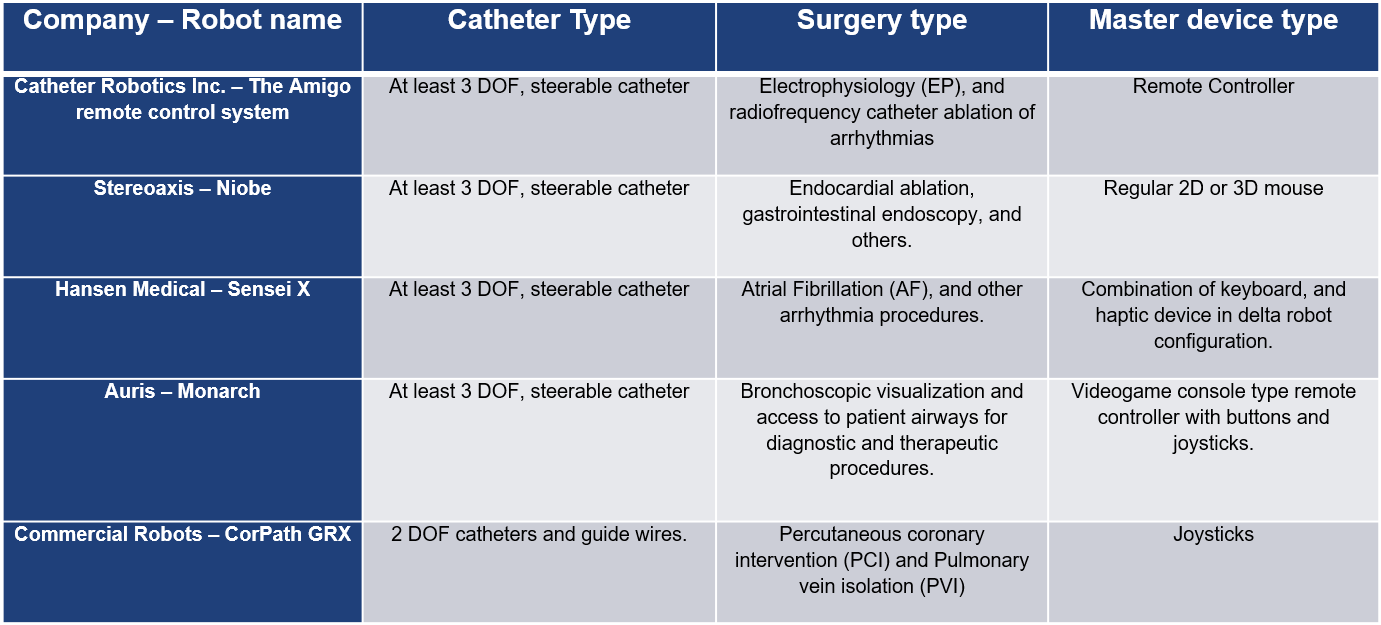
\includegraphics[width=1.0\textwidth]{img/statetable.PNG}
   \caption{Comparison between the state of the art devices in catheter teleoperation}
   \label{img:statetable}
\end{figure}

\begin{figure}[ht]
   \centering
   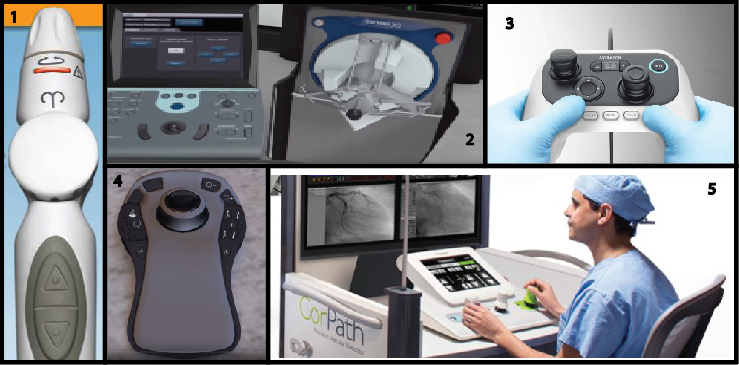
\includegraphics[width=1.0\textwidth]{img/statedevices.PNG}
   \caption{State of the art devices, (1) The Amigo Remote System, (2) Sensei X, (3) Monarch, (4) Stereoaxis and (5) CorPath GRX}
   \label{img:statedevices}
\end{figure}


